\documentclass[12pt]{article}

\usepackage{lastpage} % Required to determine the last page for the footer
\usepackage{extramarks} % Required for headers and footers
\usepackage{graphicx} % Required to insert images
\usepackage{listings} % Required for insertion of code
\usepackage{courier} % Required for the courier font
\usepackage{color}

% Margins
\topmargin=-0.45in
\evensidemargin=0in
\oddsidemargin=0in
\textwidth=6.5in
\textheight=9.0in
\headsep=0.25in

\linespread{1.1} % Line spacing

\vspace{4em}

\newcommand{\Title}{Tender document} % Assignment title
\begin{document}

	\begin{center}%
		\begin{figure}[ht!]
			\centering
			
\includegraphics{./Pictures/logo.png}
		\end{figure}
		\LARGE \bf \Title \\
		{\bf Version 1.0}\\[4em]
		\LARGE {\bf SoftServe Group }\\[1em]
		\LARGE {\bf Members:}\\[2em]
		\large
		Kgothatso Phatedi Alfred Ngako		(12236731) \\[1em]
		Tokologo “Carlo” Machaba			(12078027) \\[1em]
		Mathys Ellis						(12019837) \\[8em]
			    
	\end{center}%
				
	\newpage
		\tableofcontents
			
	\newpage
	\section{Tender options}
	\begin{enumerate}
		\item UP - Post-Doctoral Application Management system
		\item UP - Proof-Obligation Manager
		\item Cortical Systems - Financial Markets Simulation
	\end{enumerate}	
	
	\subsection{Proposal for tender option 1}
		The SoftServe group purposes a system is powered by a campus server and uses a web interface.
		This system will be completely centralised in order to allow maximum audibility, security and application management.
		Further the system will also centralise all communication between the various stakeholders. Also the web interface will be extremely simple to use so to prevent staff training and reduce applicant usage confusion. We further envision a system that will be highly flexible by creating a simple "plug in" modular process pipeline that can easily allow for the removal and addition of new features.We also want to create a system that can allow for easy integration into the current UP student and personal management system. But can also run independent of it. So to allow for future development and integration.
		
	\subsection{Proposal for tender option 2}
	N/A
	
	\subsection{Proposal for tender option 3}
	N/A	
	\newpage
	\section{Team}
	
	\subsection{CV: Mathys Ellis}
	\colorbox{green}{\makebox[475px]{}}
	
	\begin{figure}[ht!]
		\centering
		\fboxsep=0mm%padding thickness
		\fboxrule=4pt%border thickness
		\framebox{
\includegraphics[scale=0.4]{./Pictures/MathysEllis.jpg}}
	\end{figure}
		
	\begin{flushleft}
		\begin{tabbing}
			\hspace*{4cm}\=\hspace*{3cm}\kill
			\textbf{Name:} \> Mathys \\	
			\textbf{Surname:} \> Ellis \\
			\textbf{Field of Study:} \> BSc (Computer Science)
		\end{tabbing}
		
		\textbf{Contact info:}	
		\begin{itemize}
			\item Cellphone: 0734038592
			\item Email: mox.1990@gmail.com
		\end{itemize}
	
		\textbf{Skills:}
		\begin{itemize}
			\item Programming in languages such as: C++, C, Java, Delphi
			\item Database work with: MySQL, SQLserver
			\item Web Design and Implementation in: HTML, PHP, Javascript, XML
		\end{itemize}
	
		\textbf{Work Experience:}
		\begin{itemize}
			\item 2013 - 2014: Research assistant at University of Pretoria
			\item 2013: Freelance web development for Universiteitsoord-gemeente 
		\end{itemize}
	
		\textbf{Additional Info:} \\
		\vspace{0.1in}
	 	An ambitious, driven, capable and hard woking bilingual student. \\
		\vspace{0.1in}
		
		\textbf{Interests:} \\
		\vspace{0.1in}
	 	Philosophy, art, nature, video games, motorbikes, travel, languages. \\
	 	\vspace{0.1in}
	\end{flushleft}
	
	\newpage
	\subsection{CV: Alfred Ngako}
	\colorbox{green}{\makebox[475px]{}}
	
	\begin{figure}[ht!]
		\centering
		\fboxsep=0mm%padding thickness
		\fboxrule=4pt%border thickness
		\framebox{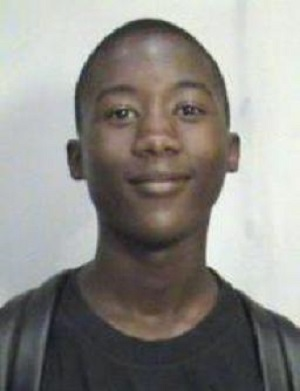
\includegraphics[scale=0.5]{./Pictures/AlfredNgako.jpg}}
	\end{figure}
		
	\begin{flushleft}
		\begin{tabbing}
			\hspace*{4cm}\=\hspace*{3cm}\kill
			\textbf{Name:} \> Kgothatso Phatedi Alfred \\	
			\textbf{Surname:} \> Ngako \\
			\textbf{Field of Study:} \> BSc (Computer Science)
		\end{tabbing}
		
		\textbf{Contact info:}	
		\begin{itemize}
			\item Cellphone: 0739383807
			\item Email: kngako@ymail.com
		\end{itemize}
		
	
	
		\textbf{Skills:}
		\begin{itemize}
			\item Programming in languages such as C++ and Java.
			\item Android App development
		\end{itemize}
	
		\textbf{Work Experience:}
		\begin{itemize}
			\item February 2012 - present: Teaching Assistant at University of Pretoria.
			\item November 2013 - present: Research assistant at University of Pretoria.
			\item June - July 2013: Contractor at CSIR.
			\item December 2013 - January 2014: Contractor at CSIR.
		\end{itemize}
	
		\textbf{Additional Info:} \\
		\vspace{0.1in}
	 	Dedicated person who works hard to ensure that results come out as positive as possible, with the knowledge that success is not an overnight event.\\
		\vspace{0.1in}
		
		\textbf{Interests:} \\
		\vspace{0.1in}
	 	Art, technology, psychology, community development and history.  \\
	 	\vspace{0.1in}
	\end{flushleft}

	\newpage
	{\subsection{CV: Tokologo Machaba}
	\colorbox{green}{\makebox[475px]{}}
	
	\begin{figure}[ht!]
		\centering
		\fboxsep=0mm%padding thickness
		\fboxrule=4pt%border thickness
		\framebox{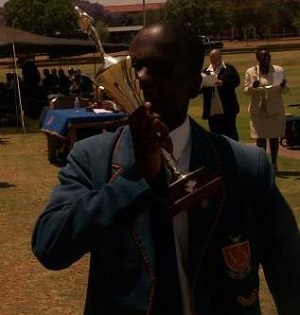
\includegraphics[scale=0.6]{./Pictures/Carlo.jpg}}
	\end{figure}
		
	\begin{flushleft}
		\begin{tabbing}
			\hspace*{4cm}\=\hspace*{3cm}\kill
			\textbf{Name:} \> Tokologo "Carlo"\\	
			\textbf{Surname:} \> Machaba \\
			\textbf{Field of Study:} \> BSc (Computer Science)
		\end{tabbing}
		
		\textbf{Contact info:}	
		\begin{itemize}
			\item Cellphone: 0832538067
			\item Email: tokomachaba@gmail.com
		\end{itemize}		
	
	
		\textbf{Skills:}
		\begin{itemize}
			\item Programming in languages such as C++ and Java.
			\item Web Development
		\end{itemize}
	
		\textbf{Work Experience:}
		\begin{itemize}
			\item July 2013 - Present: Network Administrator at Huis Taaibos.
		\end{itemize}
	
		\textbf{Additional Info:} \\
		\vspace{0.1in}
	 	Typical guy who believes sarcasm should be considered a language by itself.\\
		\vspace{0.1in}
		
		\textbf{Interests:} \\
		\vspace{0.1in}
	 Sports, music, community development, technology  \\
	 	\vspace{0.1in}
	\end{flushleft}
\end{document}
